\section{Durchführung}
\label{sec:Durchführung}
Für die Durchführung des Versuches stehen ein Frequenzgenerator, ein Oszilloskop, eine Stromquelle, ein Steckbrett und LM741 Operationsverstärker, sowie diverse Widerstände 
und Kondensatoren zur Verfügung.
Die verschiedenen Bauteile und die Pinbelegung des LM741 OpAmp's sind in \autoref{fig:aufbau} zu sehen.
\begin{figure}
    \centering
    \begin{subfigure}{.4\textwidth}
        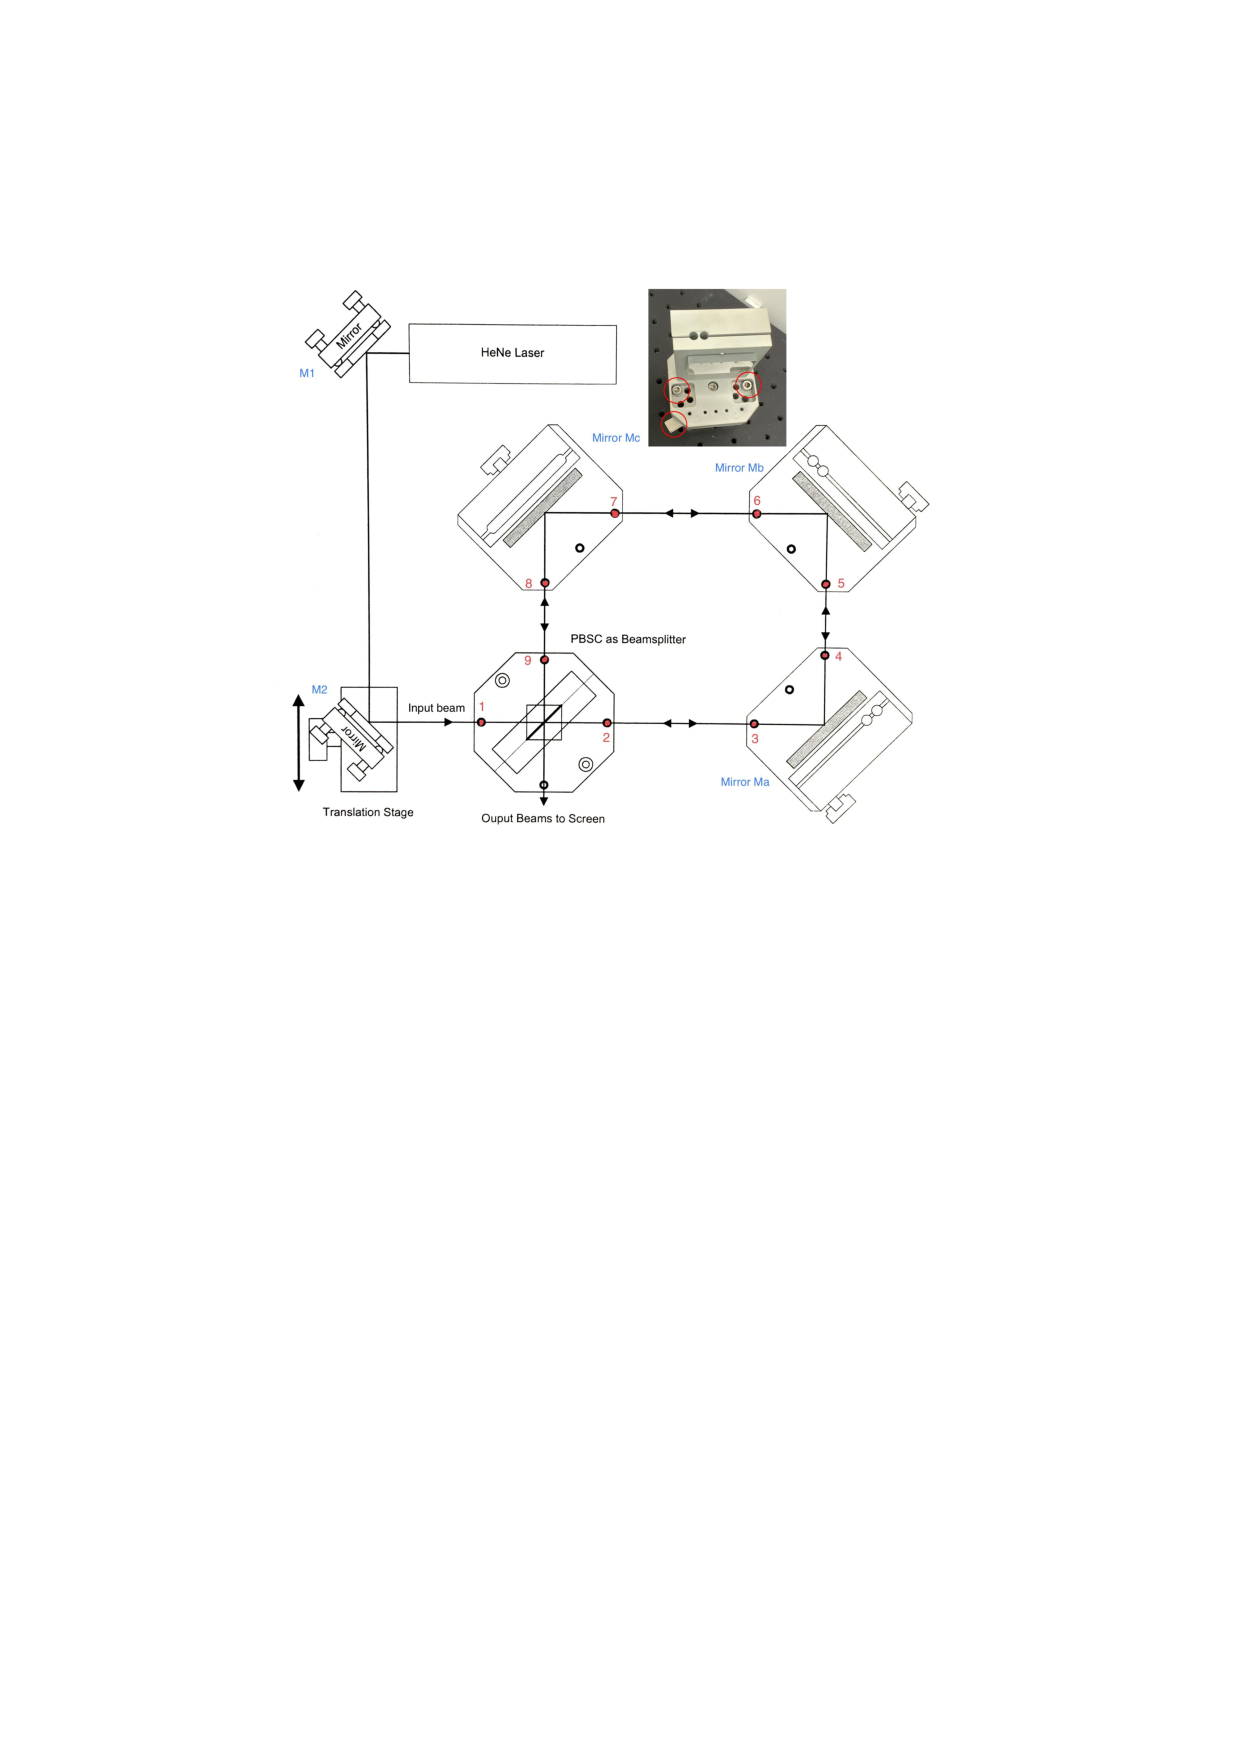
\includegraphics[width=\textwidth]{"content/pics/setup.png"}
        \caption{Verfügbare Bauteile des Versuchaufbaus \cite{v51}.}
        \label{fig:aufbau1}
    \end{subfigure}
    \hfill
    \begin{subfigure}{.4\textwidth}
        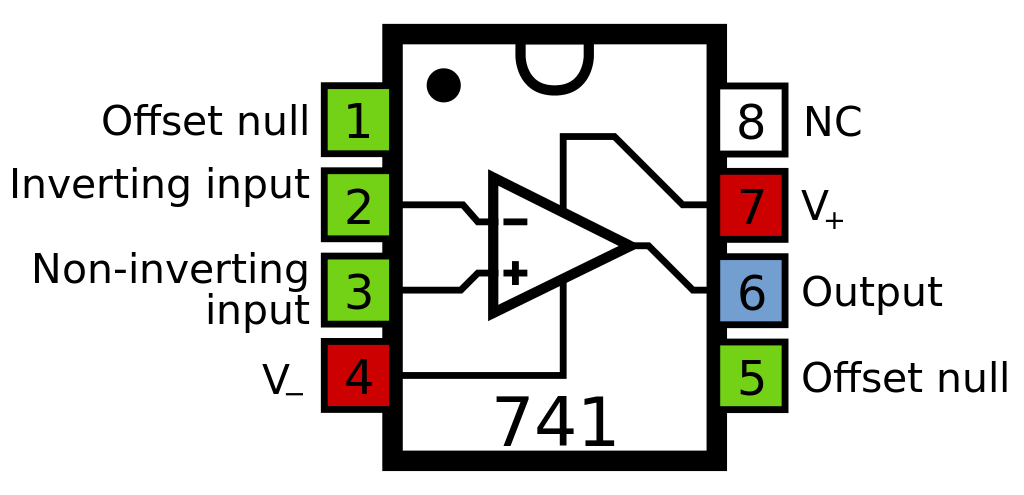
\includegraphics[width=\textwidth]{"content/pics/LM741.png"}
        \caption{Pinbelegung des LM741 Operationsverstärkers \cite{LM741}.}
        \label{fig:generator2}
    \end{subfigure}
    \caption{Bestandteile des Versuchaufbaus.}
    \label{fig:aufbau}
\end{figure}

Zuerst wird die Schaltung des invertierenden Linearverstärkers nach \autoref{fig:inverting} aufgebaut.
Es werden zuerst Widerstände $R_1 = \qty{1}{\kilo\ohm}$ und $R_2 = \qty{100}{\kilo\ohm}$ verwendet. Die Frequenzabhängigkeit der Amplitude und der Phase zwischen Eingangs- und 
Ausgangsspannung werden über mehrere Größenordnungen der Frequenz gemessen ($\qtyrange[range-phrase = -]{1}{100}{\kilo\hertz}$).
Die Messung wird für zwei weitere Konfigurationen der Widerstände wiederholt. \\
Anschließend wird der Integrator nach \autoref{fig:integrator} mit $R = \qty{10}{\kilo\ohm}$ und $C = \qty{100}{\nano\farad}$ aufgebaut. Wieder wird die Ausgangsspannung als
Funktion der Frequenz gemessen. Außerdem wird die Form des Ausgangsignals für eine Rechteck- und Dreieckspannung (und Sinusspannung) mithilfe des Oszilloskops gespeichert. 
Analoge Messungen werden für den Differenzierer nach \autoref{fig:differenzierer} mit $R = \qty{100}{\kilo\ohm}$ und $C = \qty{22}{\nano\farad}$ vorgenommen. \\
Der Schmitt-Trigger (\autoref{fig:schmitt_trigger}) wird mit $R_1 = \qty{10}{\kilo\ohm}$ und $R_2 = \qty{100}{\kilo\ohm}$ aufgebaut. Durch stetiges Erhöhen der Spannung oder 
mithilfe einer Dreieckspannung wird die Schwellenspannung der Schaltung mehrfach bestimmt und gemittelt. Des Weiteren werden Messdaten der Eingangs- und Ausgangsspannung mithilfe 
des Oszilloskops gespeichert. \\
Der Generator aus \autoref{fig:generator1} wird mit $R_1 = \qty{10}{\kilo\ohm}$, $R_1 = \qty{100}{\kilo\ohm}$, $R_1 = \qty{1}{\kilo\ohm}$ und $C = \qty{1}{\micro\farad}$
aufgebaut. Es werden $U_1$ und $U_\text{a}$ mit dem Oszilloskop gespeichert um anschließend die Frequenz und Amplitude des Generators bestimmen zu können. \\
Zuletzt wird der Generator mit variierender Amplitude (\autoref{fig:generator2}) mit  $C = \qty{22}{\nano\farad}$ oder $C = \qty{100}{\nano\farad}$ aufgebaut.
Die Dämpfung der Amplitude und die Schwingungsdauer werden mit dem Oszilloskop gemessen.
